\documentclass[11pt]{article}
\usepackage[margin = 1in]{geometry}
\usepackage{setspace}
\usepackage{amsmath}
\usepackage{amssymb}
\usepackage{amsthm}
\usepackage{graphicx}
\usepackage{enumitem}
\usepackage{url}
\usepackage[parfill]{parskip}
\usepackage{listings}
\usepackage{caption}
\usepackage{subcaption}
\usepackage[utf8]{inputenc}
\usepackage{xcolor}
\definecolor{codegreen}{rgb}{0,0.6,0}
\definecolor{codegray}{rgb}{0.5,0.5,0.5}
\definecolor{codepurple}{rgb}{0.58,0,0.82}
\definecolor{backcolour}{rgb}{0.95,0.95,0.92}
\lstdefinestyle{mystyle}{
	backgroundcolor=\color{backcolour},   
	commentstyle=\color{magenta},
	numberstyle=\tiny\color{codegray},
	stringstyle=\color{codegreen},
	basicstyle=\ttfamily\footnotesize,
	breakatwhitespace=false,         
	breaklines=true,                 
	captionpos=b,                    
	keepspaces=true,                 
	numbers=left,                    
	numbersep=5pt,                  
	showspaces=false,                
	showstringspaces=false,
	showtabs=false,                  
	tabsize=2
}
\lstset{style=mystyle}
\newcommand{\skipline}{\vspace{\baselineskip}}
\newcommand{\spacer}{\noalign{\medskip}}
\newcommand{~}{\sim}
\newcommand{\approches}{\rightarrow}
\newcommand{\qarrow}{\quad \rightarrow \quad}
\newcommand{\qqarrow}{\qquad \rightarrow \qquad}
\newcommand{\qqtext}[1]{\qquad \text{ #1 } \qquad}
\newcommand{\pard}[2]{\frac{\partial #1}{\partial #2}}
\newcommand{\answer}[1]{\textbf{\boldmath #1}}
\newenvironment{problem}[1]{\textbf{Problem #1: }}{\newpage}

\doublespacing
\begin{document}
	
	\begin{center}
		\textbf{Goppa Code Encryption Decryption} \\
		\textbf{Instructor: J.C. Interlando} \\
		\textbf{Stephen Giang RedID: 823184070} \\
		\skipline \skipline
	\end{center}

	{\Large\textbf{Introduction}}
	\\ \\
	In this project, we use sources from N.J. Patterson for his decoding algorithm of Goppa Codes along with McEliece's Public Key Encryption and Decryption methods.  Our goal for this project is to understand how binary strings are encrypted and decrpyted and model modern day texting and emailing.  This report contains all the code used to encrypt and decrypt binary strings, along with decoding Goppa Codes. We will also be coding within the University of Sydney's Magma Computational Algebra System to be doing all of our calculations.

	\newpage
	Notice the algorithm from ``The Algebraic Decoding of Goppa Codes'' by N.J. Patterson that we will use to decrypt our own Goppa Codes:
	\begin{figure}[h!]
		\centering
		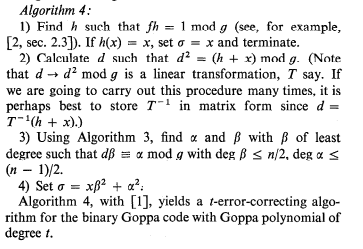
\includegraphics[height=6cm]{Alg4.png}
	\end{figure}
	\\ 
	Notice the application of the following steps from the Algorithm above that will check and correct Goppa Codes:
	\begin{enumerate}[label = (\arabic*)]
		\item \textit{Find $h$ such that $fh = 1\mod g$.  If $h(x) = x$, set $\sigma = x$ and terminate.}
		\\ \\
		We first can set up our field $F$ to be an extension of the $GF(2)$, such that $F = GF(2^m)$, for some arbitrary $m$. We also then create a Polynomial Ring of $F$ that we will denote as $R(z)$. This is a ring of polynomials with variable $z$ and coefficients within $F$.
\begin{lstlisting}[language=Java]
m:=3;											// choose some power for the creation of the field 
F<B>:=GF(2^m);						// creation of the field F (extension of GF(2)).
R<z>:=PolynomialRing(F);	// creation of the polynomial ring F[z].
\end{lstlisting}
		From here, we can choose an arbitrary irreducible in $F$ polynomial, and notate it as the Goppa Polynomial.
\begin{lstlisting}[language=Java]
// Goppa Polynomial with variable z and coefficients in F(B^n)
G:= z^3 + B*z^2 + z + 1;
\end{lstlisting}
		From here, we find its locator set, a subset of $F$ such that $G(x) \not = 0$ for all $x \in F$.
\begin{lstlisting}[language=Java]
// Creates the locator set of the Goppa Code
L:= [x : x in F | Evaluate(G,x) ne 0];
\end{lstlisting}
		From here, we notate the following: $r = \deg(G)$, $n =$ length of the locator set which is also the length of the code, $k \geq n - mr$ is the lower bound for the dimension of the Goppa Code, $d \geq r + 1$ is the minimum distance.
\begin{lstlisting}[language=Java]
r:= Degree(G);    	// Degree of G
n:= #L;             // Length of locator set, and length of code
k:= n - m*r;        // Lower Bound for Dimension of Goppa Code
d:= r + 1;          // Minimum Distance
\end{lstlisting}
		We choose an arbitrary binary word, $C$ of length $n$ that we will be decoding and correcting:
\begin{lstlisting}[language=Java]
// Choose a random word C
C:=[Random(0,1) : i in [1..n]];
\end{lstlisting} 
	
		From here, we now need notate $S_0 = \frac{1}{z - \beta_i}$ to be an array of the multiplicative inverse of $z - \beta_i$, where $\beta_i \in L$.
\begin{lstlisting}[language=Java]
// Finds the Multiplicative inverse of z - beta_i in G
S0:= [Modinv(z - L[i], G) : i in [1..n]];
\end{lstlisting}
		We now find the syndrome of $C$, $R_a$, with parity check matrix $S_0$.  This is also denoted as $f$ in this algorithm.
\begin{lstlisting}[language=Java]
// Ra is the syndrome of C, with parity check matrix S0
Ra:=0;
for i in [1..n] do
	Ra:=Ra + (S0[i] * C[i]);
end for;
\end{lstlisting}
		We can check to see if $C$ is a Goppa code by seeing whether or not the syndrome multiplied with the parity check matrix is $0\mod G$.
\begin{lstlisting}[language=Java]
// Check to see if C is a goppa codeword.
GoppaCheck:= Ra mod G eq 0;
\end{lstlisting}
		From here, assuming C is not a codeword, we calculate the multiplicative inverse of $R_a$ and denote it as $h$.
\begin{lstlisting}[language=Java]
// Multiplicative inverse of the Syndrome Ra or f in Pattersons
h:=Modinv(Ra,G);
\end{lstlisting}
		\item \textit{Calculate $d$ such that $d^2 = (h+x)\mod g.$ (Note that $d \rightarrow d^2 \mod g$ is a linear transformation, $T$ say. If we are going to carry out this procedure many times, it is perhaps best to store $T^{-1}$ in matrix form since $d = T^{-1}(h+x)$.)}
		\\ \\
		Here it is asking us to find $d$ such that it is the square root of $h + x \mod G$. Notice a general example using some polynomial $v$:
		\begin{align*}
			v^{2^{mr}} &\equiv v \mod G  & v^{2^{mr} * (2^{-1})} &\equiv (v)^{1/2} \mod G \\
			(v^{2^{mr}})^{1/2} &\equiv (v)^{1/2} \mod G & v^{2^{mr-1}} &\equiv \sqrt{v} \mod G
		\end{align*}
		So using this, we can get $d$ to be the following:
		\[d = (h+z)^{2^{mr - 1}} \mod G\]
		However, for large values of $mr$, we get \textit{Argument too large} errors.  To combat this, we can square $(h + z)$ and then mod it by G $mr  - 1$ times, as shown below:
\begin{lstlisting}[language=Java]
d := (h + z);
for i in [1..(m*r - 1)] do
	d := d^2 mod G;
end for;
\end{lstlisting}
		\newpage
		\item \textit{Using Algorithm 3, find $\alpha$ and $\beta$ with $\beta$ of least degree such that $d\beta \equiv \alpha \mod g$ with $\deg \beta \leq n/2, \deg \alpha \leq (n-1)/2$.}
		\\ \\
		Notice the Euclidean Algorithm between $G$ and $d$:
		\begin{align*}
			G &= dq_1 + r_1 \\
			d &= r_1q_2 + r_2 \\
			\vdots & \vdots \\
			r_n &= r_{n-1}q_n 
		\end{align*}	
		Notice, we can find intermediate values of the following equation from:
		\[\nu G + \mu d = GCD(G,d) \qqarrow s_i G + t_i d = r_i\]
		Using the following $q$ values, we can solve for $t_i$ and $r_i$ which represents $\beta$ and $\alpha$ respectively:
		\[t_i = t_{i-1}q_{i-1} + t_{i-2}\]
		and $r_i$ is found from the Euclidean Algorithm.
\begin{lstlisting}[language=Java]
function EuclideanAlgorithm(G, d)
	ng := Degree(G);    // Degree of G
	t_im2 := R!0;       // t_0 = 0
	t_im1 := R!1;       // t_1 = 1
	t_i := t_im1;       // t_i = t_{i-1}
	r_i := d;
	
	// Check degrees to see if we can stop function
	if Degree(t_i) le Floor(ng/2) and Degree(r_i) le Floor((ng-1)/2) then
		return r_i, t_i;
	else
	repeat
		q, r_i := Quotrem(G, d); 
		if r_i ne 0 then 
			G := d; 
			d := r_i; 
			// t_i = q t_{i-1} + t_{i-2}
			t_i := q * t_im1 + t_im2; 
			// Increment i by 1
			t_im2 := t_im1; 
			t_im1 := t_i; 
		end if;  
	until Degree(t_i) le Floor(ng/2) and Degree(r_i) le Floor((ng-1)/2);
		return r_i, t_i;
	end if;
end function;  

// Step 3
alpha, beta := EuclideanAlgorithm(G, d);
\end{lstlisting}
		\item \textit{Set $\sigma = x\beta^2 + \alpha^2$.}
\begin{lstlisting}[language=Java]
// Step 4
sigma := z*beta^2 + alpha^2;
\end{lstlisting}
	From here, the roots of $\sigma$ show the locations of the errors:
\begin{lstlisting}[language=Java]
roots:= Roots(sigma);
\end{lstlisting}
	\end{enumerate}

	\newpage
	
	Notice the following example:
\begin{lstlisting}[language=Java]
function EuclideanAlgorithm(G, d)
	ng := Degree(G);    // Degree of G
	t_im2 := R!0;       // t_0 = 0
	t_im1 := R!1;       // t_1 = 1
	t_i := t_im1;       // t_i = t_{i-1}
	r_i := d;
	
	// Check degrees to see if we can stop function
	if Degree(t_i) le Floor(ng/2) and Degree(r_i) le Floor((ng-1)/2) then
		return r_i, t_i;
	else
	repeat
		q, r_i := Quotrem(G, d); 
		if r_i ne 0 then 
			G := d; 
			d := r_i; 
			// t_i = q t_{i-1} + t_{i-2}
			t_i := q * t_im1 + t_im2; 
			// Increment i by 1
			t_im2 := t_im1; 
			t_im1 := t_i; 
		end if;  
	until Degree(t_i) le Floor(ng/2) and Degree(r_i) le Floor((ng-1)/2);
	return r_i, t_i;
	end if;
end function; 
\end{lstlisting}
\newpage
\begin{lstlisting}[language=Java]
m:=3;                           // choose some power for the creation of the field 
F<B>:=GF(2^m);                    // creation of the field F (extension of GF(2)).
R<z>:=PolynomialRing(F);          // creation of the polynomial ring F[z].

// GoppaPolynomial with variable z and coefficients in F (B^n)
// For this we make our own Polynomial
G:= z^3 + B*z^2 + z + 1;

// Creates the locator set of the Goppa Code
L:= [x : x in F | Evaluate(G,x) ne 0];

r:= Degree(G);    // Degree of G
n:= #L;                // Length of locator set, and length of code
k:= n - m*r;        // Lower Bound for Dimension of Goppa Code
d:= r + 1;            // Minimum Distance

// Finds the Multiplicative inverse of z - beta_i in G
S0:= [Modinv(z - L[i], G) : i in [1..n]];

// Choose a random codeword C
C:=[Random(0,1) : i in [1..n]];

// Ra is the syndrome of C, with parity check matrix S0
Ra:=0;
for i in [1..n] do
Ra:=Ra + (S0[i] * C[i]);
end for;

// Check to see if C is a goppa codeword.
GoppaCheck:= Ra mod G eq 0;

// Multiplicative inverse of the Syndrome Ra or f in Pattersons
h:=Modinv(Ra,G);

// Step 2
d:=(h + z)^(2^(m*r - 1) ) mod G;

// Step 3
alpha, beta := EuclideanAlgorithm(G, d);

// Step 4
sigma := z*beta^2 + alpha^2;

// Show everything given:
print "F: ", F;
print "R: ", R;
print "G: ", G;
print "G is Irreducible: ", IsIrreducible(G);
print "L: ", L;
print "Degree of G: ", r;
print "Code Length: ", n;
print "Lower Bound for Dimension: ", k;
print "Minimum Distance: ", d;
print "S0: ", S0;
print "C: ", C;
print "Ra: ", Ra;
print "C is a Goppa Code: ", GoppaCheck;
print "h: ", h;
print "d: ", d;
print "alpha: ", alpha;
print "beta: ", beta;
print "sigma: ", sigma;
print "roots: ", roots;	
\end{lstlisting}

\newpage

\begin{lstlisting}[language=Java]
F:  Finite field of size 2^3
R:  Univariate Polynomial Ring in z over GF(2^3)
G:  z^3 + B*z^2 + z + 1
G is Irreducible:  true
L:  [ 0, 1, B, B^2, B^3, B^4, B^5, B^6 ]
Degree of G:  3
Code Length:  8
Lower Bound for Dimension:  -1
Minimum Distance:  B^2*z^2 + B^4*z + B^5
S0:  [
z^2 + B*z + 1,
B^4*z^2 + z + B^5,
B^4*z^2 + B^4,
B^2*z^2 + B^6*z + B^4,
B^2*z^2 + B^2*z + B^3,
B^5*z^2 + z + 1,
B^6*z^2 + B^5*z + B^4,
B^2*z^2 + z + 1
]
C:  [ 1, 0, 0, 1, 0, 0, 0, 1 ]
Ra:  z^2 + B^4*z + B^4
C is a Goppa Code:  false
h:  z^2 + B^2
d:  B^2*z^2 + B^4*z + B^5
alpha:  B^5*z
beta:  B^5*z + B^2
sigma:  B^3*z^3 + B^3*z^2 + B^4*z
roots:  [ <0, 1>, <B^2, 1>, <B^6, 1> ]
\end{lstlisting}

	\newpage
	
	Now that we have our decoding algorithm, we can implement McEliece Public-Key Encryption and Decryption methods.
	\begin{figure}[h!]
		\centering
		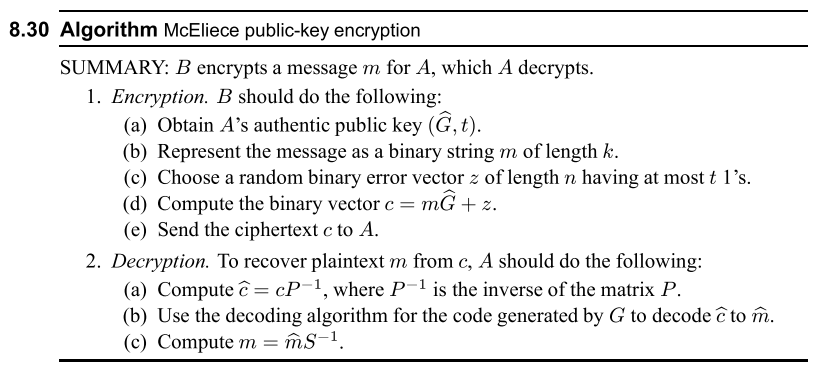
\includegraphics[height=7cm, width=\linewidth]{Alg830.png}
	\end{figure}
	\\ \\
	With the following variables described below:
	\begin{figure}[h!]
		\centering
		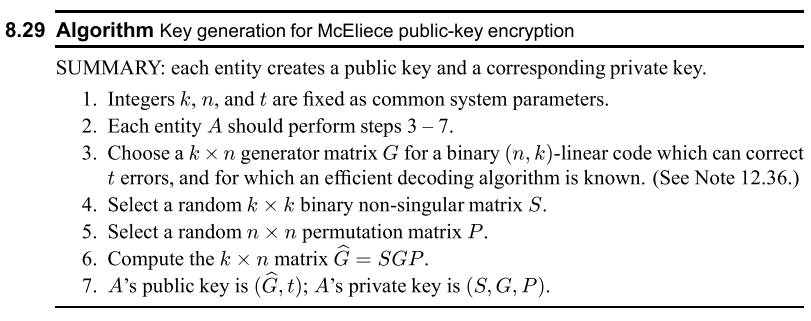
\includegraphics[height=7cm, width=\linewidth]{Alg829.png}
	\end{figure}
	\newpage
	I begin by setting a value $mField$ that will be set and used for the creation of our field, $F$
\begin{lstlisting}[language=Java]
mField := 3;
\end{lstlisting}
	We then set our field, polynomial ring, and set our generator polynomial dependent on different values of $mField$.
\begin{lstlisting}[language=Java]
F<B> := GF(2^mField);                   
R<z> := PolynomialRing(F);

if mField eq 3 then
	Gpoly := B^2*z^2 + z + B^3;
end if;
if mField eq 4 then
	Gpoly := B^14*z^3 + B^10*z^2 + B^9*z + B^13;
end if;
if mField eq 5 then
	Gpoly := B^18*z^6 + B^18*z^5 + B^26*z^4 + B^8*z^3 + B^26*z^2 + B^16*z + B^15;
end if;
if mField eq 6 then
	Gpoly := B^24*z^3 + B^59*z^2 + B^47*z + B^57;
end if;
if mField eq 7 then
	Gpoly := B^57*z^15 + B^14*z^14 + B^101*z^13 + B^17*z^12 + B^83*z^11 + B^9*z^10 + B^52*z^9 + B^64*z^8 + B^25*z^7 + B^74*z^6 + B^59*z^5 + B^43*z^4 + B^94*z^3 + B^105*z^2 + B^59*z + B^60;
end if;
\end{lstlisting}
	\newpage
	From here, we construct $L, G, S, P, \hat{G}$, which are the Locator Set, Generator Matrix of $Gpoly$ with size $k \times n$, a random nonsingular matrix of size $k \times k$, a random Permutation matrix of size $n \times n$, a public key matrix of size $k \times n$, respectively. Where $k$ is the dimension of our code, $C$, and $n$ is the length of our code.  Also to the generator matrix, $G$, we take note of the columns that contain the columns of the $k \times k$ identity matrix.
\begin{lstlisting}[language=Java]
L := [x : x in F | Evaluate(Gpoly,x) ne 0];
r := Degree(Gpoly);
n := #L;  
C := GoppaCode(L, Gpoly);
k := Dimension(C);

G := GeneratorMatrix(C);
G := Matrix(R,G);
identityIndicies := leftIdentity(G,k,n);

S := RandomGLnZ(k, 2, 3);
S := Matrix(R, S);

Q := randomPermuation(n);
P := PermutationMatrix(R, Q);

Ghat := S*G*P;
\end{lstlisting}
	Earlier we had tried to make a random nonsingular matrix with the following while loop:
\begin{lstlisting}[language=Java]
repeat
	S:=[Random(0,1) : i in [1..k^2]];
	S:=Matrix(R,k,k,S);
until IsSingular(S) eq false;
\end{lstlisting}
	This, however, would be the bottle neck to our algorithm for large values of $k$.  This is due to the check for singularity computing determinants of very large matrices.  Luckily we have a Magma function that can calculate for us a random nonsingular matrix.
\begin{lstlisting}[language=Java]
S := RandomGLnZ(k, 2, 3);
S := Matrix(R, S);
\end{lstlisting}
	\newpage
	Now, we can start the encryption process. We choose to send a binary message, $m$ of length $k$.  We then multiply it with $\hat{G}$ and add $z$, a vector with length $n$, that will have weight at most the degree of $Gpoly$.  This will produce for us, $c$, the encrypted message.
\begin{lstlisting}[language=Java]
m := [Random(0,1) : i in [1..k]];
m := Matrix(R,1,k,m);

z:= [0: i in [1..n]];
weight := Random(1, r);
for i in [1..weight] do
	repeat
		index := Random(1,n);
	until z[index] eq 0;
	z[index] := z[index] + 1;
end for;
z:=Matrix(R,1,n,z);

c:= m*Ghat + z;
\end{lstlisting}
	From here, we start our decryption process.  We take our encrypted message, $c$, and multiply it with $P^{-1}$.  We then use our decoding algorithm of Goppa Codes, and use it to find the error locations, or errorIndicies.  Once corrected, we can take the $k$ columns from $identityIndicies$, to get us $\hat{m}$.  Lastly, we multiply it with $S^{-1}$ to get our original message.
\begin{lstlisting}[language=Java]
chat:=c*(P^-1);

errorIndicies:=GoppaError(chat,Gpoly, mField);
mhat:=chat;
if #errorIndicies gt 0 then
	for i in [1..#errorIndicies] do
		mhat[1,errorIndicies[i]]:=mhat[1,errorIndicies[i]] + 1;
	end for;
end if;
mhat := Submatrix(mhat, [1..1], identityIndicies);

mDecrypted:=mhat*(S^-1);
\end{lstlisting}  

	\newpage
	Notice the following example and its output:
\begin{lstlisting}[language=Java]
function GoppaError(C, G, m)
	F<B>:=GF(2^m);
	R<z>:=PolynomialRing(F);
	L:= [x : x in F | Evaluate(G,x) ne 0];
	r:= Degree(G);
	n:= #L;
	k:= n - m*r;
	d:= r + 1;
	
	S0:= [Modinv(z - L[i], G) : i in [1..n]];
	Ra:=0;
	for i in [1..n] do
		Ra:=Ra + (S0[i] * C[1,i]);
	end for;
	
	// Check to see if C is a goppa codeword.
	GoppaCheck:= Ra mod G eq 0;
	
	
	if GoppaCheck eq false then
	
		h:=Modinv(Ra,G);
		d := (h + z);
		for i in [1..(m*r - 1)] do
			d := d^2 mod G;
		end for;
		
		function EuclideanAlgorithm(G, d)
			ng := Degree(G);    // Degree of G
			t_im2 := R!0;       // t_0 = 0
			t_im1 := R!1;       // t_1 = 1
			t_i := t_im1;       // t_i = t_{i-1}
			r_i := d;
			
			if Degree(t_i) le Floor(ng/2) and Degree(r_i) le Floor((ng-1)/2) then
				return r_i, t_i;
			else
			repeat
				q, r_i := Quotrem(G, d); 
				if r_i ne 0 then 
					G := d; 
					d := r_i; 
					// t_i = q t_{i-1} + t_{i-2}
					t_i := q * t_im1 + t_im2; 
					// Increment i by 1
					t_im2 := t_im1; 
					t_im1 := t_i; 
				end if;  
			until Degree(t_i) le Floor(ng/2) and Degree(r_i) le Floor((ng-1)/2);
			return r_i, t_i;
			end if;
		end function; 
		
		alpha, beta := EuclideanAlgorithm(G, d);
		sigma := z*beta^2 + alpha^2;
		roots := Roots(sigma);
		if #roots gt 0 then
			index := 1;
			errorIndicies := [0 : i in [1..#roots]];
			for j in [1..#roots] do
				for i in [1..#L] do
					if L[i] eq roots[j,1] then
						errorIndicies[j] := i;
					end if;
				end for;
			end for;
			return errorIndicies;
		end if;
		return [];
		end if;
	return []; 
end function;

function leftIdentity(G, k, n)
	indicies := [0 : i in [1..k]];
	index := 1;
	for j in [1..n] do
		rest := true;
		for i in [1..k] do
			if i ne index and G[i][j] eq 1 then
				rest := false;
			end if;
		end for;
		if rest eq true and G[index][j] eq 1 then
			indicies[index] := j;
			index := index + 1;
			if index gt k then
				break;
			end if;
		end if;
	end for;
	
	return indicies;
end function;

function randomPermuation(n)
	Q := [0 : i in [1..n]];
	for i in [1..n] do
		repeat
			a := Random(1,n);
		until (a in Q) eq false;
		Q[i] := a;
	end for;
	return Q;
end function;
\end{lstlisting}
\newpage
\begin{lstlisting}[language=Java]
function EncryptRandomMessage(mField, printDetails)
	F<B> := GF(2^mField);                   
	R<z> := PolynomialRing(F);
	
	if mField eq 3 then
		Gpoly := B^2*z^2 + z + B^3;
	end if;
	if mField eq 4 then
		Gpoly := B^14*z^3 + B^10*z^2 + B^9*z + B^13;
	end if;
	if mField eq 5 then
		Gpoly := B^18*z^6 + B^18*z^5 + B^26*z^4 + B^8*z^3 + B^26*z^2 + B^16*z + B^15;
	end if;
	if mField eq 6 then
		Gpoly := B^24*z^3 + B^59*z^2 + B^47*z + B^57;
	end if;
	if mField eq 7 then
		Gpoly := B^57*z^15 + B^14*z^14 + B^101*z^13 + B^17*z^12 + B^83*z^11 + B^9*z^10 + B^52*z^9 + B^64*z^8 + B^25*z^7 + B^74*z^6 + B^59*z^5 + B^43*z^4 + B^94*z^3 + B^105*z^2 + B^59*z + B^60;
	end if;
	
	
	L := [x : x in F | Evaluate(Gpoly,x) ne 0];
	r := Degree(Gpoly);
	n := #L;  
	C := GoppaCode(L, Gpoly);
	k := Dimension(C);
	
	G := GeneratorMatrix(C);
	G := Matrix(R,G);
	identityIndicies := leftIdentity(G,k,n);
	
	S := RandomGLnZ(k, 2, 3);
	S := Matrix(R, S);
	
	Q := randomPermuation(n);
	P := PermutationMatrix(R, Q);
	
	Ghat := S*G*P;
	
	m := [Random(0,1) : i in [1..k]];
	m := Matrix(R,1,k,m);
	
	z:= [0: i in [1..n]];
	weight := Random(1, r);
	for i in [1..weight] do
		repeat
			index := Random(1,n);
		until z[index] eq 0;
		z[index] := z[index] + 1;
	end for;
	z:=Matrix(R,1,n,z);
	
	c:= m*Ghat + z;
	
	if printDetails then
		print " ----- ";  
		print "Gpoly: ", Gpoly;
		print " ----- ";  
		print "r: ", r;
		print " ----- ";  
		print "n: ", n;
		print " ----- ";  
		print "k: ", k;
		print " ----- ";
		print "G: ", G;
		print " ----- ";
		print "S: ", S;
		print " ----- ";
		print "P: ", P;
		print " ----- ";
		print "Ghat: ", Ghat;
		print " ----- ";
		print "m: ", m;
		print " ----- ";
		print "z: ", z;
		print " ----- ";
		print "c: ", c;
	end if;
	
	return c, mField, S, G, P, Gpoly, identityIndicies, m;

end function;

function DecryptRandomMessage(c, mField, S, G, P, Gpoly, identityIndicies, printDetails)
	chat:=c*(P^-1);
	errorIndicies:=GoppaError(chat,Gpoly, mField);
	mhat:=chat;
	if #errorIndicies gt 0 then
		for i in [1..#errorIndicies] do
			mhat[1,errorIndicies[i]]:=mhat[1,errorIndicies[i]] + 1;
		end for;
	end if;
	mhat := Submatrix(mhat, [1..1], identityIndicies);
	
	mDecrypted:=mhat*(S^-1);
	
	if printDetails then
		print " ----- ";
		print "chat: ", chat;
		
		print " ----- ";
		print "mhat: ", mhat;
		
		print " ----- ";
		print "mDecrypted: ", mDecrypted;
	end if;
	
	return mDecrypted;
end function;

mField := 4;
c, mField, S, G, P, Gpoly, identityIndicies, m := EncryptRandomMessage(mField,true);
mDecrypted := DecryptRandomMessage(c, mField, S, G, P, Gpoly, identityIndicies, true);

if (m eq mDecrypted) then
print "SUCCESS";
else
print "FAILURE: LOOK FOR ERRORS";
end if;


\end{lstlisting}
\newpage
\begin{lstlisting}[language=Java]
-----
Gpoly:  B^14*z^3 + B^10*z^2 + B^9*z + B^13
-----
r:  3
-----
n:  16
-----
k:  4
-----
G:
[1   0   0   1   1   0   0   0   1   0   1   1   1   0   0   1]
[0   1   0   1   0   1   1   0   0   1   1   1   1   0   1   1]
[0   0   1   0   1   0   1   0   0   1   0   0   1   1   0   1]
[0   0   0   0   0   0   0   1   0   0   1   1   1   1   1   1]
-----
S:
[   1    0    0    0]
[   0    1    0    1]
[   0    0    1    0]
[   0    0    0    1]
-----
P:
[0   0   0   0   0   0   0   1   0   0   0   0   0   0   0   0]
[0   1   0   0   0   0   0   0   0   0   0   0   0   0   0   0]
[0   0   0   0   0   0   0   0   0   0   0   0   0   1   0   0]
[0   0   1   0   0   0   0   0   0   0   0   0   0   0   0   0]
[0   0   0   0   0   0   0   0   0   0   0   0   0   0   1   0]
[0   0   0   0   0   0   0   0   1   0   0   0   0   0   0   0]
[0   0   0   0   0   1   0   0   0   0   0   0   0   0   0   0]
[0   0   0   0   0   0   0   0   0   0   0   0   1   0   0   0]
[0   0   0   0   0   0   1   0   0   0   0   0   0   0   0   0]
[0   0   0   0   0   0   0   0   0   0   1   0   0   0   0   0]
[1   0   0   0   0   0   0   0   0   0   0   0   0   0   0   0]
[0   0   0   1   0   0   0   0   0   0   0   0   0   0   0   0]
[0   0   0   0   0   0   0   0   0   0   0   1   0   0   0   0]
[0   0   0   0   0   0   0   0   0   1   0   0   0   0   0   0]
[0   0   0   0   1   0   0   0   0   0   0   0   0   0   0   0]
[0   0   0   0   0   0   0   0   0   0   0   0   0   0   0   1]
-----
Ghat:
[1   0   1   1   0   0   1   1   0   0   0   1   0   0   1   1]
[0   1   1   0   0   1   0   0   1   1   1   0   1   0   0   0]
[0   0   0   0   0   1   0   0   0   1   1   1   0   1   1   1]
[1   0   0   1   1   0   0   0   0   1   0   1   1   0   0   1]
-----
m:
[   1    0    0    1]
-----
z:
[1   0   0   0   0   0   0   0   0   0   0   0   0   0   0   0]
-----
c:
[1   0   1   0   1   0   1   1   0   1   0   0   1   0   1   0]
-----
chat:
[1   0   0   1   1   0   0   1   1   0   1   0   0   1   1   0]
-----
mhat:
[   1    0    0    1]
-----
mDecrypted:
[   1    0    0    1]
SUCCESS
\end{lstlisting}
	\newpage
	
	{\Large\textbf{Conclusion and Findings}}
	\\ \\
	Some early challenges with this project was a lack of knowledge on specific topics about Algebraic Coding Theory.
	\\ \\
	I can say that this encryption and decryption process came out to be only about 60\% effective initially. This was due to the fact that I was swapping columns of G, which is not allowed.  Another hurdle within the project was that Magma could not compute the algorithm because of runtime errors, when $mField > 5$. When using our decoding algorithm, we needed to calculate $d = (h + z)^{2^{mr - 1}}$. When $m  = 5$, we use a generator polynomial of degree $r = 6$.  This will result in $d = (h + z)^{536870912}$, which our Magma cannot handle.  However, we found a work around this, and that was to square $(h + z)$ then modulo it with $G$, a total of $mr  - 1$ times.  We discovered a bottle neck issue that arose which was that our earlier method of finding $S$ took too long computationally because it was very computation heavy on finding the determinant of a large $k \times k$ matrix.  We found a work around this using Magma's own random matrix generator that was indeed nonsingular already.  With all of those fixes, we can now run our algorithm to 100\% efficiency. 
	\\ \\
	I found this research project to be very enticing, and very informative as towards how messaging works in terms of security. This also allowed me to build my skills towards implementing and adjusting algorithms. 
	\\ \\
	Also I would like to very much thank my Professor, J.C Interlando, for his commitment to me as a student, and truly being a kindhearted figure towards me in such a trying time. Thank you so much Professor!
	
\end{document}
